\subsection{Data samples}
\label{sec:data_sample}

The analysis uses the full 2016 $pp$ collisions data (periods A-L) with the integrated luminosity of 32.8 $\mathrm{fb^{-1}}$. In this search, because the standard ATLAS track reconstruction does not provide good sensitivity for long-lived particles, a dedicated stream, \texttt{DRAW\_RPVLL}, is used to reconstruct events using the non-standard reconstruction algorithm discussed in Section~\ref{sec:large_radius_tracking}. The stream is used in several Exotics and SUSY analyses, searching for long-lived particles. %non-standard reconstruction objects.

In \texttt{DRAW\_RPVLL} stream, a subset of events from the main physics stream is selected by \texttt{RPVLL} filters. The filters select events using High-Level Triggers (HLT) and offline selections configured for each analysis. The triggers and offline selection used in this search is discussed in Section~\ref{sec:signal_selection}. The selected events are passed downstream for reconstruction. The data is in \texttt{RAW} format so that low-level information such as detector hits can be used for the special reconstruction algorithms to reconstruct displaced tracks and vertices.
%The low-level data available in \texttt{RAW} data, such as detector hits, allows the special reconstruction algorithms to reconstruct displaced tracks and displaced vertices.

The selected events are centrally processed with AMI tag \texttt{r8669}. The dedicated track reconstruction algorithm, the \textit{large radius tracking}, and the secondary vertex reconstruction algorithm, \texttt{VrtSecInclusive}, are used to reconstruct displaced tracks and vertices, respectively. The output of \texttt{DRAW\_RPVLL} stream is in \texttt{DAOD\_RPVLL} format which is a standard \texttt{xAOD} data format with additional displaced tracks and secondary vertices reconstructed. 

The \texttt{DAOD\_RPVLL} is further processed to produce the \texttt{DAOD\_SUSY15} derivation with \texttt{AODfix} and data reduction as recommended by the Analysis Model Study Group (AMSG)~\cite{Catmore:1543445}. Table~\ref{table:data_samples} summarizes datasets used in this search.

\begin{table}[!htb]
  \centering
  \begin{tabular}{ l l }
    \hline
    \hline
    Format     				& Dataset       													\\
    \hline
	\texttt{DRAW\_RPVLL}	& data16\_13TeV.*.physics\_Main.merge.DRAW\_RPVLL.f*\_m*			\\
	\texttt{DAOD\_RPVLL}	& data16\_13TeV.*.physics\_Main.recon.DAOD\_RPVLL.f*\_r8669			\\
	\texttt{DAOD\_SUSY15}	& data16\_13TeV.*.physics\_Main.recon.DAOD\_RPVLL.f*\_r8669\_p2950	\\
    \hline
    \hline
  \end{tabular}
  \caption{Dataset used in \texttt{DRAW\_RPVLL}, \texttt{DAOD\_RPVLL}, and \texttt{DAOD\_SUSY15} format.}
  \label{table:data_samples}
\end{table}

This search uses a modified version of the standard \texttt{GoodRunsList} because a small number of events selected by \texttt{DRAW\_RPVLL} was not reconstructed successfully. The corresponding lumi blocks were removed from the \texttt{GoodRunsList}\footnote{\texttt{data16\_13TeV.periodAllYear\_DetStatus-v83-pro20-15\_DQDefects-00-02-04\_PHYS\_StandardGRL\_All\_Good\\\_25ns\_DAOD\_RPVLL\_r8669.xml}}.

\subsection{MC samples}
\label{sec:mc_sample}

\subsubsection{Signal samples}
\label{sec:signal_sample}
The long-lived $Z'$ is generated using \texttt{PYTHIA 6.4}~\cite{1126-6708-2006-05-026} in which $Z'$ is singly produced from $q\bar{q}$ scattering and decays to a $\mu\mu$, $ee$, or $e\mu$ pair. The proper lifetime, $c\tau$, is set to 100 mm, 250 mm, or 500 mm. The mass of $Z'$ is set between 100 and 1000 GeV. A width based on relativistic Breit-Wigner is assumed for the new resonance. A sample of 20k events are generated for each mass and lifetime. Table~\ref{table:MC_signal_samples} summarizes dataset identifiers (DIDs), mass, and lifetime of the signal MC samples used in this search.

\begin{table}[!htb]
  \centering
  \begin{tabular}{ c c c c c c c }
    \hline
    \hline
           &   &    & \multicolumn{3}{c}{DID}                 \\
    $m_{Z'}$ (GeV) & $\Gamma$ (GeV) & $c\tau$ (mm) &$\mu\mu$ & $ee$ & $e\mu$ \\
    \hline
    100			   &	2.8         &   100	& 308264	& 309539		&	309554		\\
    100			   &	2.8         &   250	& 308265	& 309540		&	309555		\\
    100			   &	2.8         &   500	& 308266	& 309541		&	309556		\\
    250			   &   6.9	        &   100	& 301911	& 309542		&	309557		\\
    250			   &	6.9         &   250	& 301912	& 309543		&	309558		\\
    250			   &	6.9         &   500	& 301913	& 309544		&	309559		\\
    500			   &   14.7         &   100	& 301914	& 309545		&	309560		\\
    500			   &	14.7        &   250	& 301915	& 309546		&	309561		\\
    500			   &	14.7        &   500	& 301916	& 309547		&	309562		\\
    750			   &	23.0        &   100	& 308285	& 309548		&	309563		\\
    750			   &	23.0        &   250	& 308286	& 309549		&	309564		\\
    750			   &	23.0        &   500	& 308287	& 309550		&	309565		\\
    1000	       &	31.0        &   100	& 301917	& 309551		&	309566		\\
    1000	       &	31.0        &   250	& 301918	& 309552		&	309567		\\
    1000	       &	31.0        &   500	& 301919	& 309553		&	309568		\\
    \hline
    \hline
  \end{tabular}
  \caption{Mass, lifetime, and DID of the signal MC samples.}
  \label{table:MC_signal_samples}
\end{table}
%\begin{table}[!htb]
%  \centering
%  \begin{tabular}{ c c c c c c c }
%    \hline
%    \hline
%           &   &    & \multicolumn{3}{c}{DID}                 \\
%    $m_{Z'}$ (GeV) & $\Gamma$ (GeV) & $c\tau$ (mm) & $\sigma$ (pb) &$\mu\mu$ & $ee$ & $e\mu$ \\
%    \hline
%    100			   &	2.8         &   100	& 1104 & 308264	& -		&	-		\\
%    100			   &	2.8         &   250	& 1104 & 308265	& -		&	-		\\
%    100			   &	2.8         &   500	& 1104 & 308266	& -		&	-		\\
%    250			   &   6.9	        &   100	& 64.60 & 301911	& -		&	-		\\
%    250			   &	6.9         &   250	& 64.04 & 301912	& -		&	-		\\
%    250			   &	6.9         &   500	& 64.14 & 301913	& -		&	-		\\
%    500			   &   14.7         &   100	& 5.773 & 301914	& -		&	-		\\
%    500			   &	14.7        &   250	& 5.769 & 301915	& -		&	-		\\
%    500			   &	14.7        &   500	& 5.747 & 301916	& -		&	-		\\
%    750			   &	23.0        &   100	& 1.236 & 308285	& -		&	-		\\
%    750			   &	23.0        &   250	& 1.236 & 308286	& -		&	-		\\
%    750			   &	23.0        &   500	& 1.236 & 308287	& -		&	-		\\
%    1000	       &	31.0        &   100	& 0.3902 & 301917	& -		&	-		\\
%    1000	       &	31.0        &   250	& 0.3902 & 301918	& -		&	-		\\
%    1000	       &	31.0        &   500	& 0.3848 & 301919	& -		&	-		\\
%    \hline
%    \hline
%  \end{tabular}
%  \caption{Mass, lifetime, and DID of the signal MC samples.}
%  \label{table:MC_signal_samples}
%\end{table}

The signal MC samples generated by \texttt{PYTHIA} are processed to include detector simulation using the AMI tags \texttt{s2698} and \texttt{s2726}. The samples are overlaid with simulated minimum-bias events to model multiple interactions (pile-up) in data samples. In the signal MC samples, the average number of pile-ups, $\langle\mu\rangle$, ranges from 10 to 40 with small number of events having $\langle\mu\rangle$ < 10. The difference in the $\langle\mu\rangle$ distributions between MC and data samples are corrected for by pile-up reweighting in Section~\ref{sec:efficiency_reweighting}. The resulting MC samples, in \texttt{HITS} format, are reconstructed using AMI tag \texttt{r8788}.

In the reconstruction process, the large radius tracking and \texttt{VrtSecInclusive} algorithms are used with the same configuration as data samples discussed in Section~\ref{sec:data_sample}, to reconstruct displaced tracks and vertices. The reconstructed events are stored in \texttt{DAOD\_RPVLL}, and the samples are processed to produce the \texttt{DAOD\_SUSY15} derivation with \texttt{AODfix} and data reduction. 

The representative plots of truth-level $p_{T}$ and $\eta$ distributions of $Z'$ and the muons from the decay of $Z'$, referred as \textit{signal} muons, are shown in Figure~\ref{fig:truth_zp_muon} using the signal MC samples with $m=$ 500, 1000 GeV and $c\tau=$ 100 mm. The signal MC samples with $ee$ and $e\mu$ final states produce similar distributions as shown in Appendix~\ref{app:signal_truth}.

%The $\eta$ distribution of $Z'$ shows a forward distribution, and it is reweighted to a flat $\eta$ distribution to provide model-independent result. The details are discussed in Section~\ref{sec:efficiency_reweighting}.
The $\eta$ distribution of signal muons shows that most of the signal muons are produced within the detector acceptance ($\eta <$ 2.7). The characteristic upper edge in the $p_{T}$ spectrum is related to the $Z'$ mass.
%The $p_{T}$ distribution of muons shows that muon $p_{T}$ is constrained by the $Z'$ mass.


\begin{figure}[!htb]
    \centering
    \subfloat[]{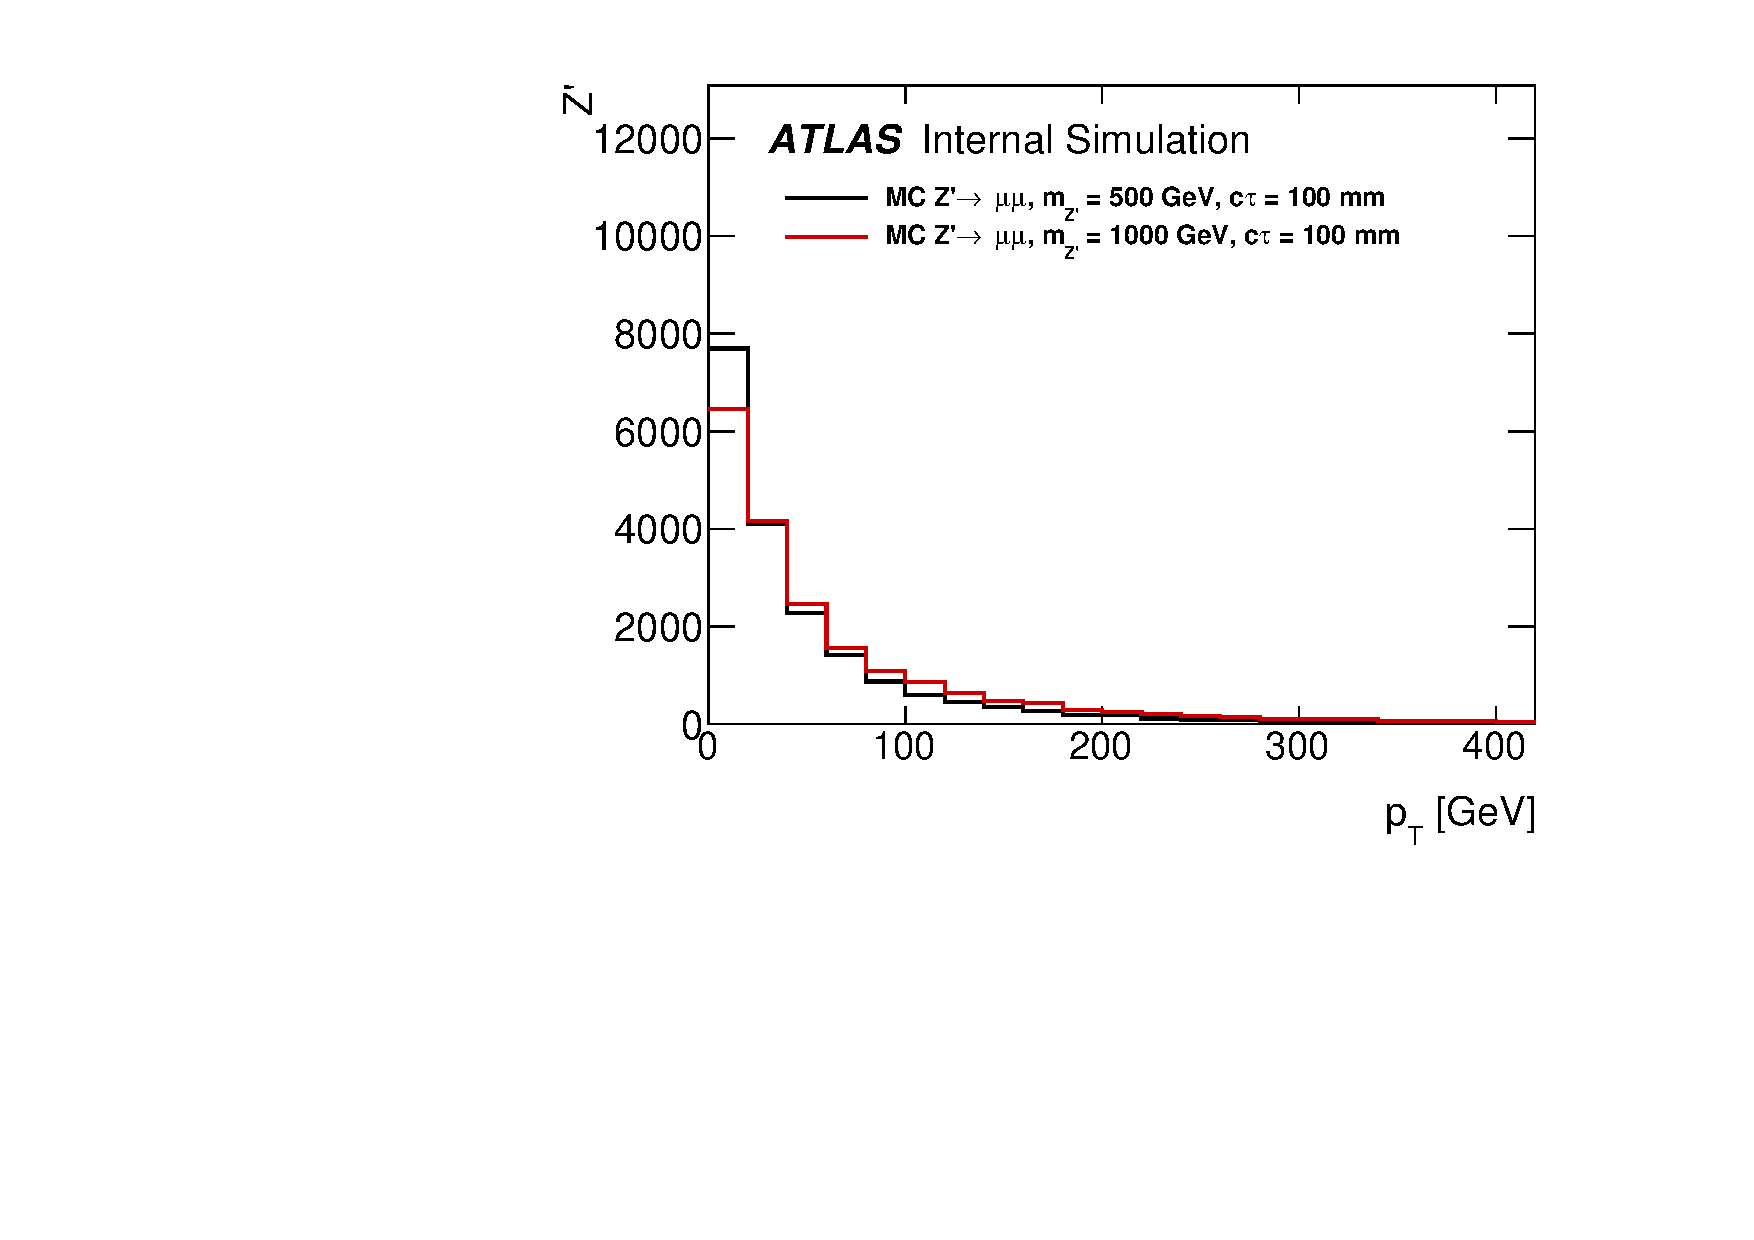
\includegraphics[width=0.45\textwidth]{figures/m_truth_zp_pt.pdf}}
    \subfloat[]{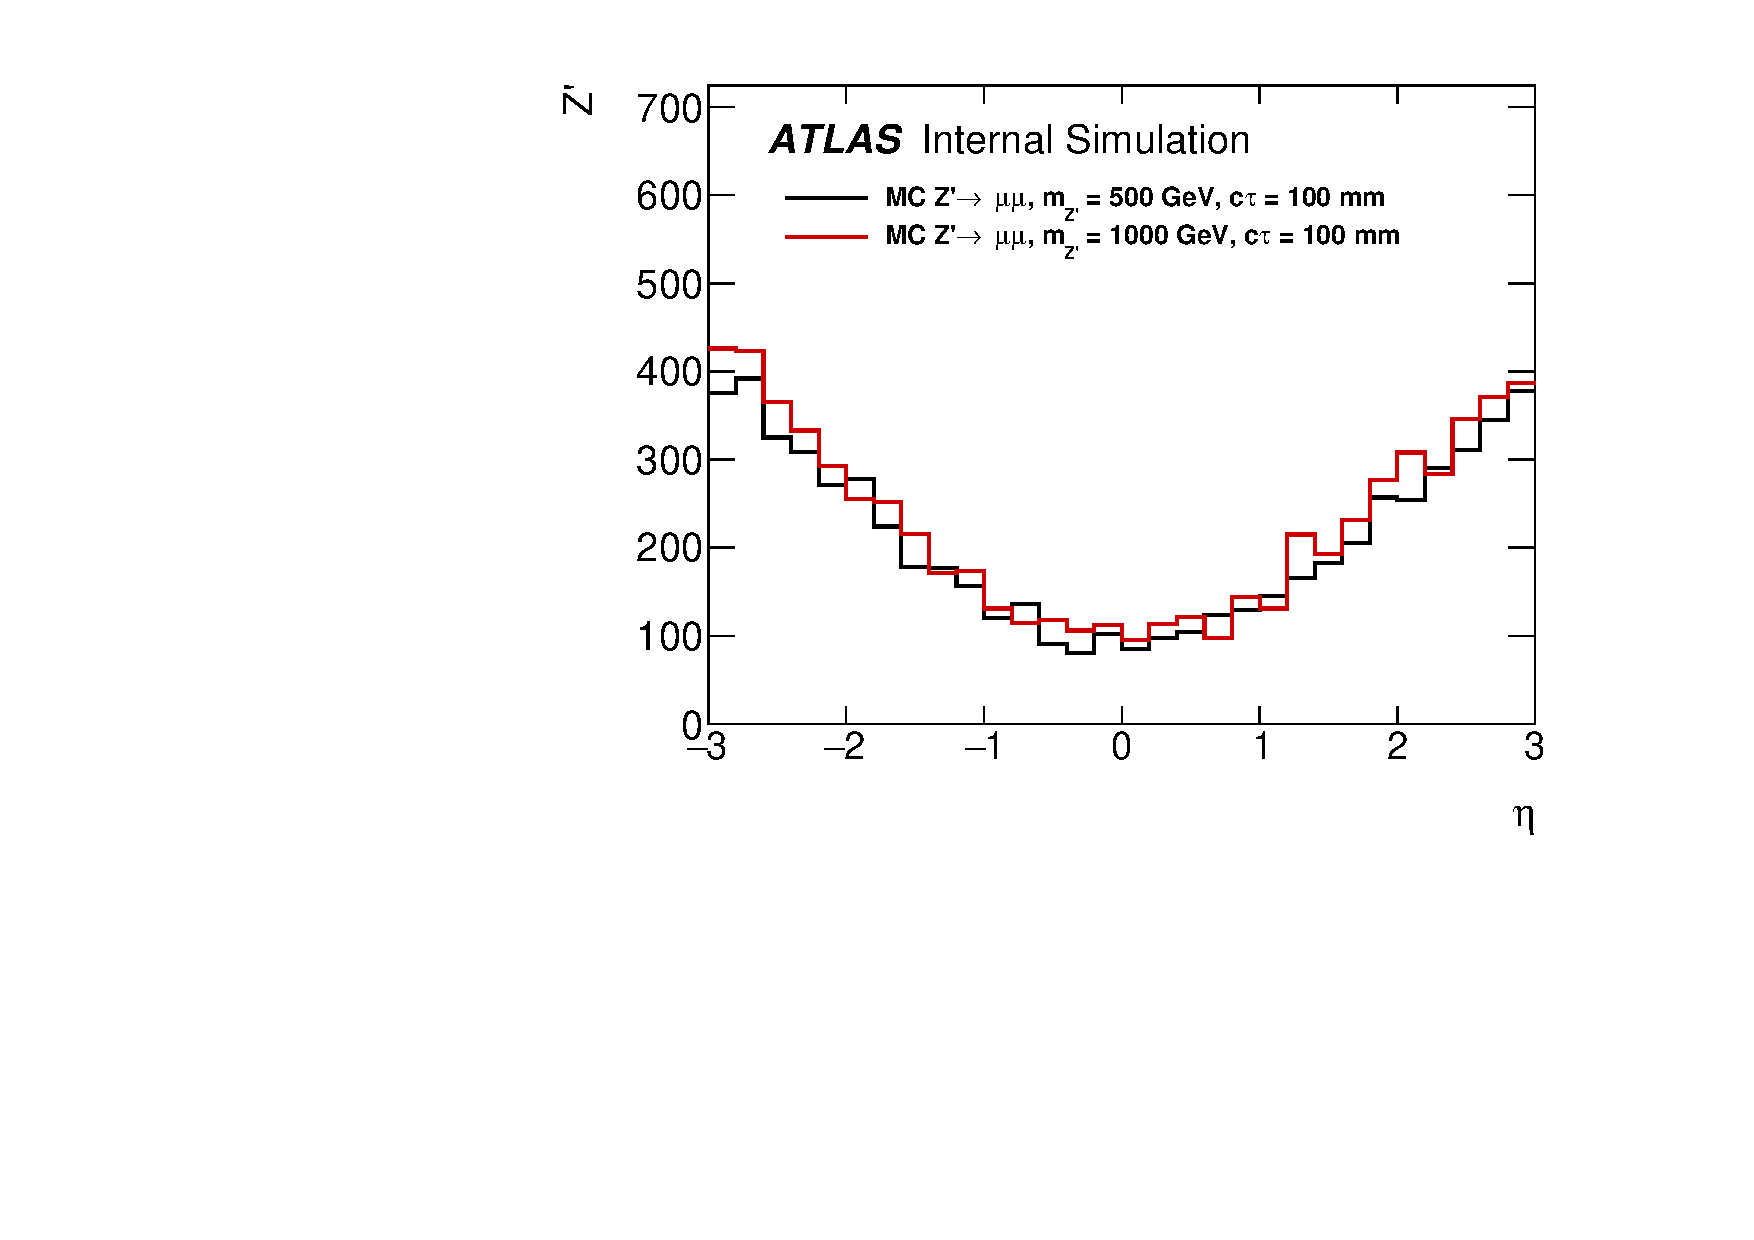
\includegraphics[width=0.45\textwidth]{figures/m_truth_zp_eta.pdf}} \\
    \subfloat[]{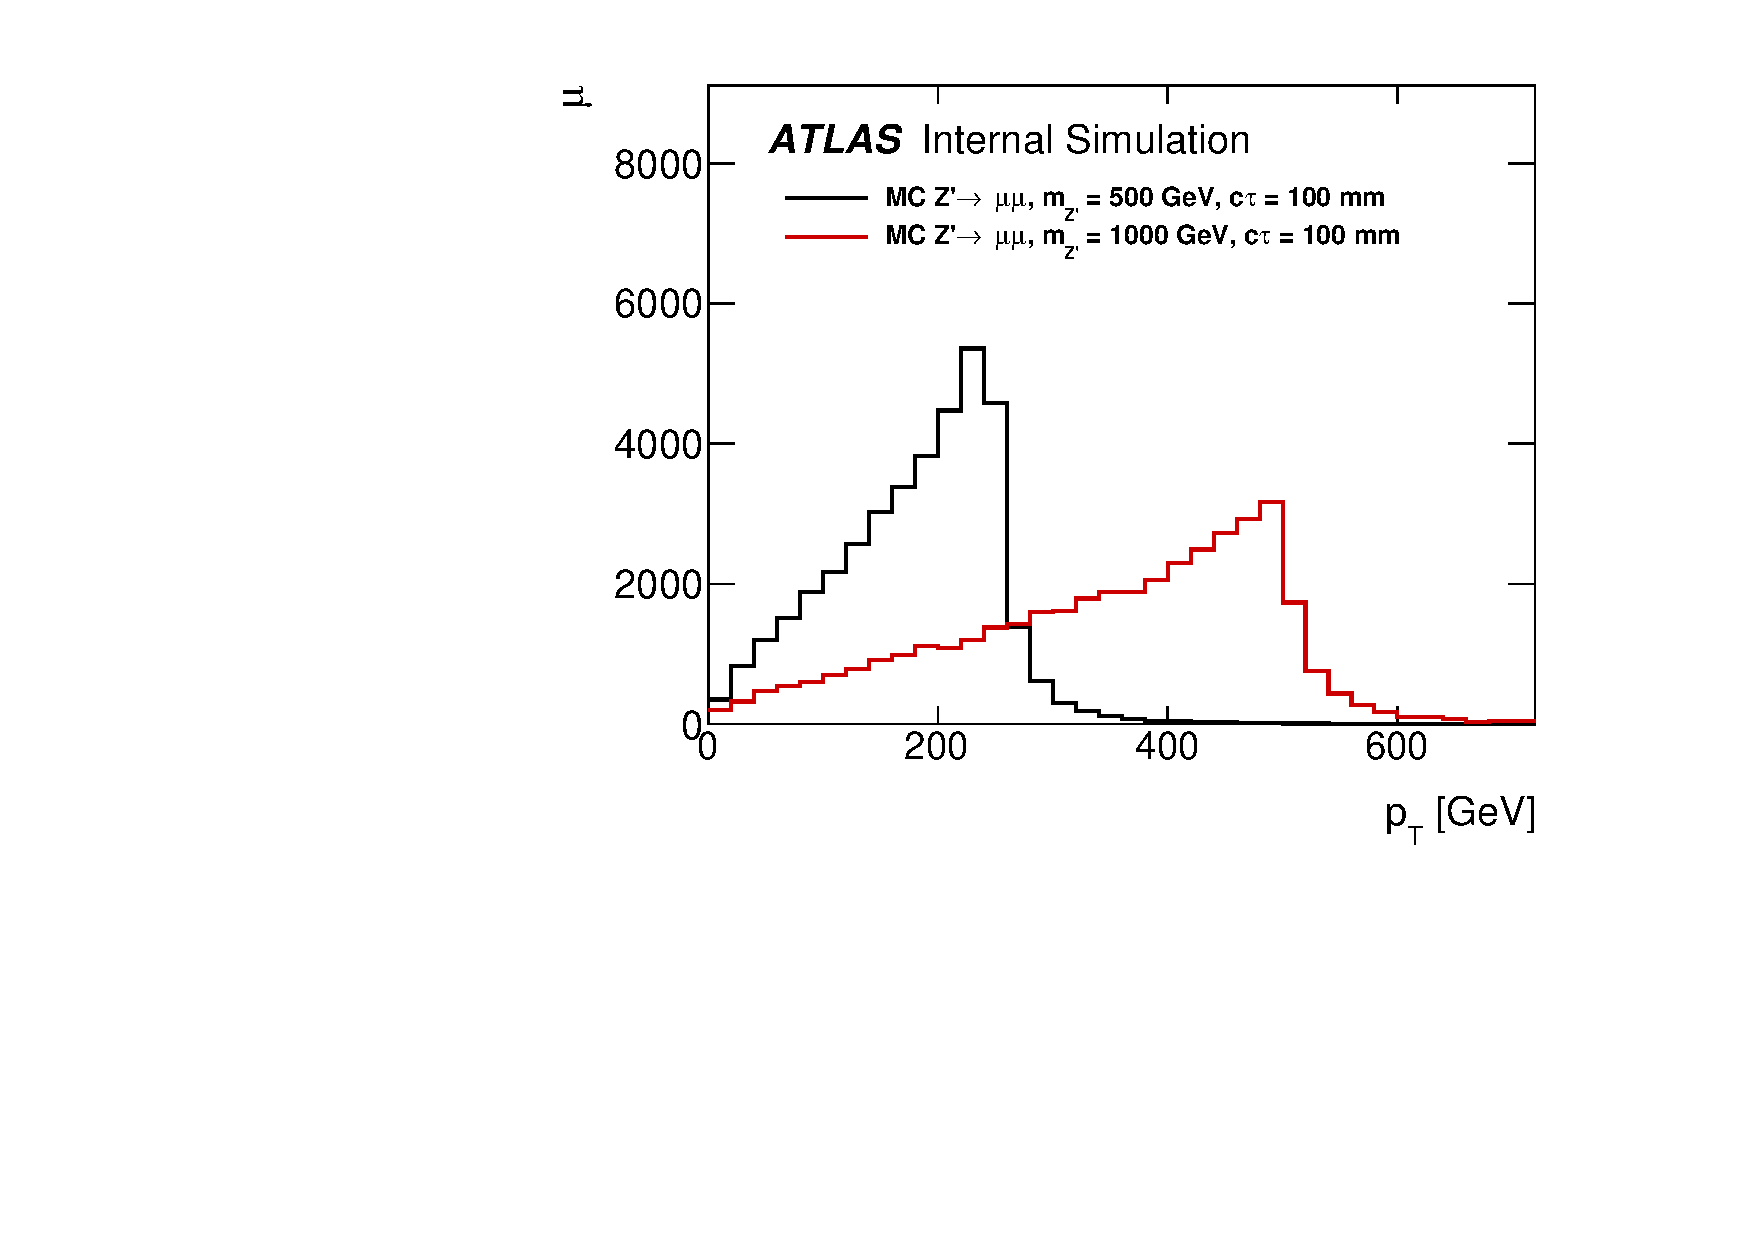
\includegraphics[width=0.45\textwidth]{figures/m_truth_muon_pt.pdf}}
    \subfloat[]{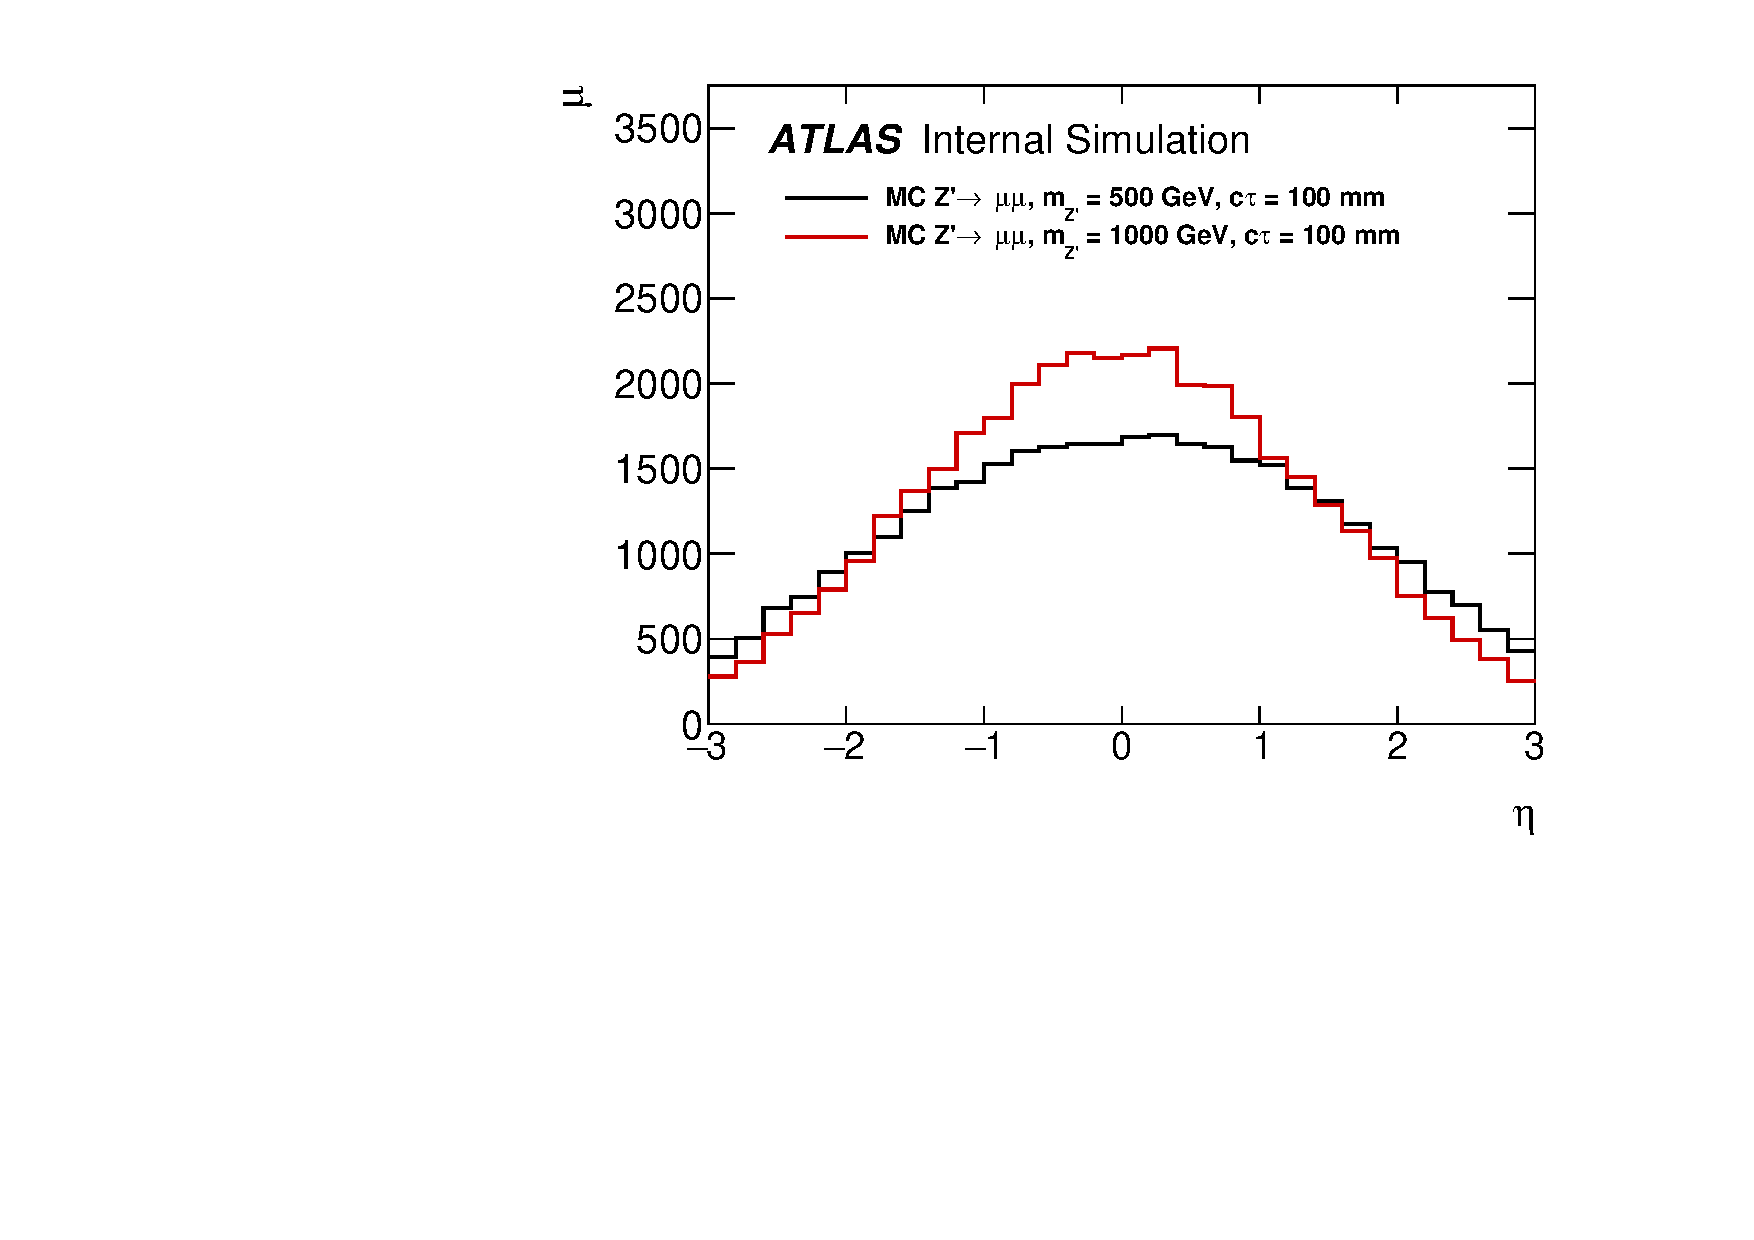
\includegraphics[width=0.45\textwidth]{figures/m_truth_muon_eta.pdf}}
    \caption{The representative plots of truth-level (a) $p_{T}$ and (b) $\eta$ distributions of $Z'$, and (c), (d) are the corresponding distributions for the signal muons. The signal MC samples are generated with $m=$ 500, 1000 GeV, and $c\tau=$ 100 mm.}
    \label{fig:truth_zp_muon}
\end{figure}


\subsubsection{Background MC samples}
\label{sec:background_mc_sample}
In this analysis, backgrounds are estimated from data because most of the backgrounds are expected to be originated from non-collision processes such as cosmic rays or random-crossing of tracks. %sources other than the SM collision process 

However, SM background samples are used to study the performance of random-crossing background estimation in Section~\ref{sec:background_estimation} and to estimate the systematic uncertainties in vertexing and tracking in Section~\ref{sec:syst}. The SM background samples are reprocessed from \texttt{HITS} using the same configuration as the signal MC sample for consistency.

The background MC samples used for background and systematic uncertainty estimations are summarized in Table~\ref{table:background_MC}.


\begin{table}[!htb]
  \centering
  \begin{tabular}{ l l l l l}
    \hline
    \hline
    Process         &   DID     &   $\sigma$ (pb)       & Events ($10^{6}$) &   $\mathcal{L}_{Int} (\mathrm{fb^{-1}})$ \\
    \hline
    $t\bar{t}$                              &   410252  &   87.8   &   0.70        &   7.97                 \\
    $ZZ\rightarrow \ell \ell \ell \ell$     &   361063  &   11.7   &   0.12        &   10.3                 \\
    $W^{-}Z\rightarrow \ell \ell \ell v$    &   361064  &   1.68   &   0.020       &   10.2                 \\
    $W^{+}Z\rightarrow \ell \ell \ell v$    &   361066  &   2.33   &   0.70        &   30.0                 \\
    $WW \rightarrow \ell \ell vv$           &   361068  &   12.8   &   0.025       &   1.95                 \\
    JZ3W                                    &   361023  &   8.45$\cdot10^{3}$      &   0.20  &   0.0247     \\
    JZ4W                                    &   361024  &   135    &   0.20        &   1.48                 \\
    JZ5W                                    &   361025  &   4.20   &   0.20        &   47.6                 \\
    JZ6W                                    &   361026  &   2.42$\cdot10^{-2}$     &   0.20  &   826        \\
    \hline
    \hline
  \end{tabular}
  \caption{Background MC samples used in the study of random-crossing background and in the estimation of tracking and vertexing systematic uncertainty.}
  \label{table:background_MC}
\end{table}
